\ifdefined\THESIS
    \chapter{\uppercase{Analysis of Distance to Contacts}}
\else
    \section{Analysis of Distance to Contacts}
\fi

% FIXME: For each subsection finding (e.g., "What is the distribution of
% contacts?") you need to add more intuition/analysis. Walk the reader through
% each figure. Highlight some actual numbers from the figures in the text. Tell
% us what those numbers mean. Tell me what I should learn. You do some of this
% already, but it really needs to be expanded. Remember, your reader is not as
% on top of this material as you are, so you need to do more handholding.

% FIXME: For all figs, I think you may need a black/white legible version. I'm
% worried about readers seeing lots of lines and not wanting to go back to the
% screen PDF to tell the difference. What did Backstrom do for their FB paper?

% FIXME: For all figs, you might want to add a takeaway sentence in the
% caption. So if a reader only looks at the fig (without following along in the
% text), they can learn something.

Every user who has multiple contacts will have some contacts who are much
closer than others. In order to estimate the locations of users, we would like
to find out which users are most likely to live nearby.  In this section, we
investigate how various types of contacts correlate with proximity.
All of the analysis in this section was done on the contacts of 249584 geo-located users.
Contacts with a predicted location error that was greater than or equal to 1000
miles were filtered out.

\subsection{What type of contact is closest?}
\label{sec:EdgeTypes}

\begin{figure}[tb]
\centering
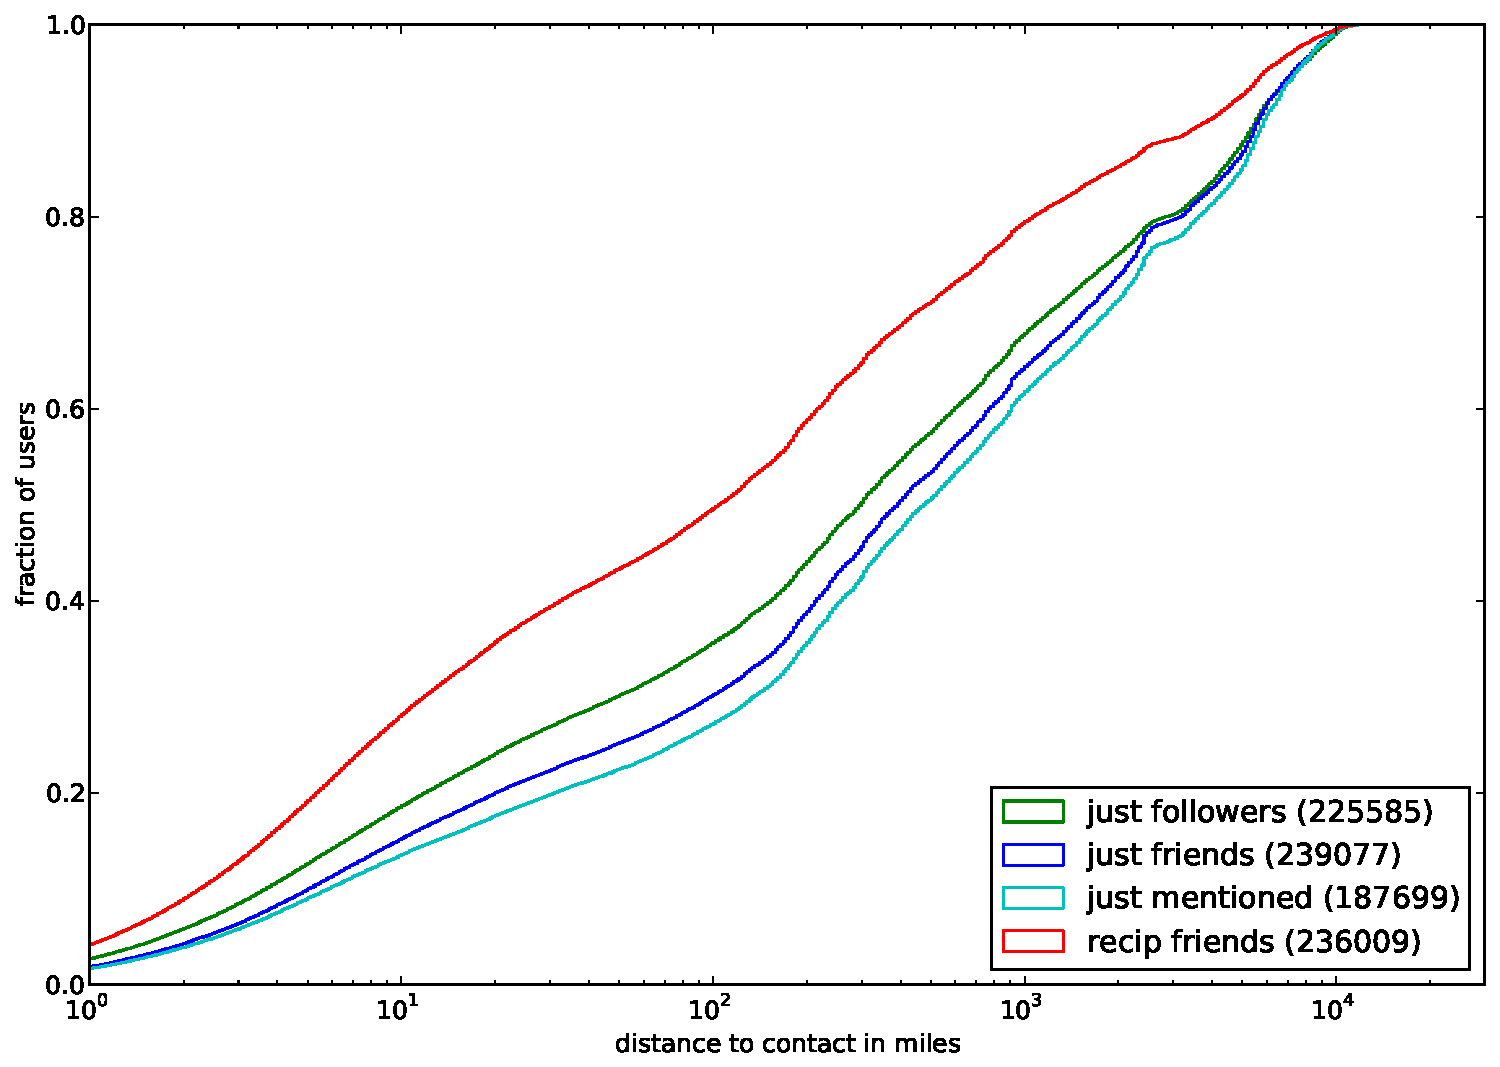
\includegraphics[width=\linewidth]{figures/edge_types_cuml.pdf}
\caption{
CDF of distance from geo-located users to users they have some contact
with.
}
\label{fig:EdgeTypesCum}
\end{figure}

FIXME: add US-only line to one of these graphs for comparison to other papers

Figure~\ref{fig:EdgeTypesCum} shows the cumulative distribution
function(CDF) of the distance between a geo-located user and several types of
contacts.
Distance is plotted on a logarithmic scale to show both local and
global effects.

In general, reciprocal friends are the closest, followed by followers, friends,
and finally users who are just mentioned.
37\% of reciprocal friends live within 25 miles while only 18\% of users
who are just mentioned live within that radius.
While it may seem that since being followed by someone and following someone
should be identical, they are not.
Celebrity and news accounts on Twitter often have large numbers of followers,
but they normally do not follow a large number of users.
Since the geo-located user was selected randomly, they are usually an average
user and not a celebrity.
If they follow someone, it might be a celebrity; however, if someone follows
them, it is probably someone who knows them.

\subsection{What is the distribution of contacts?}

\begin{figure}[tb]
\centering
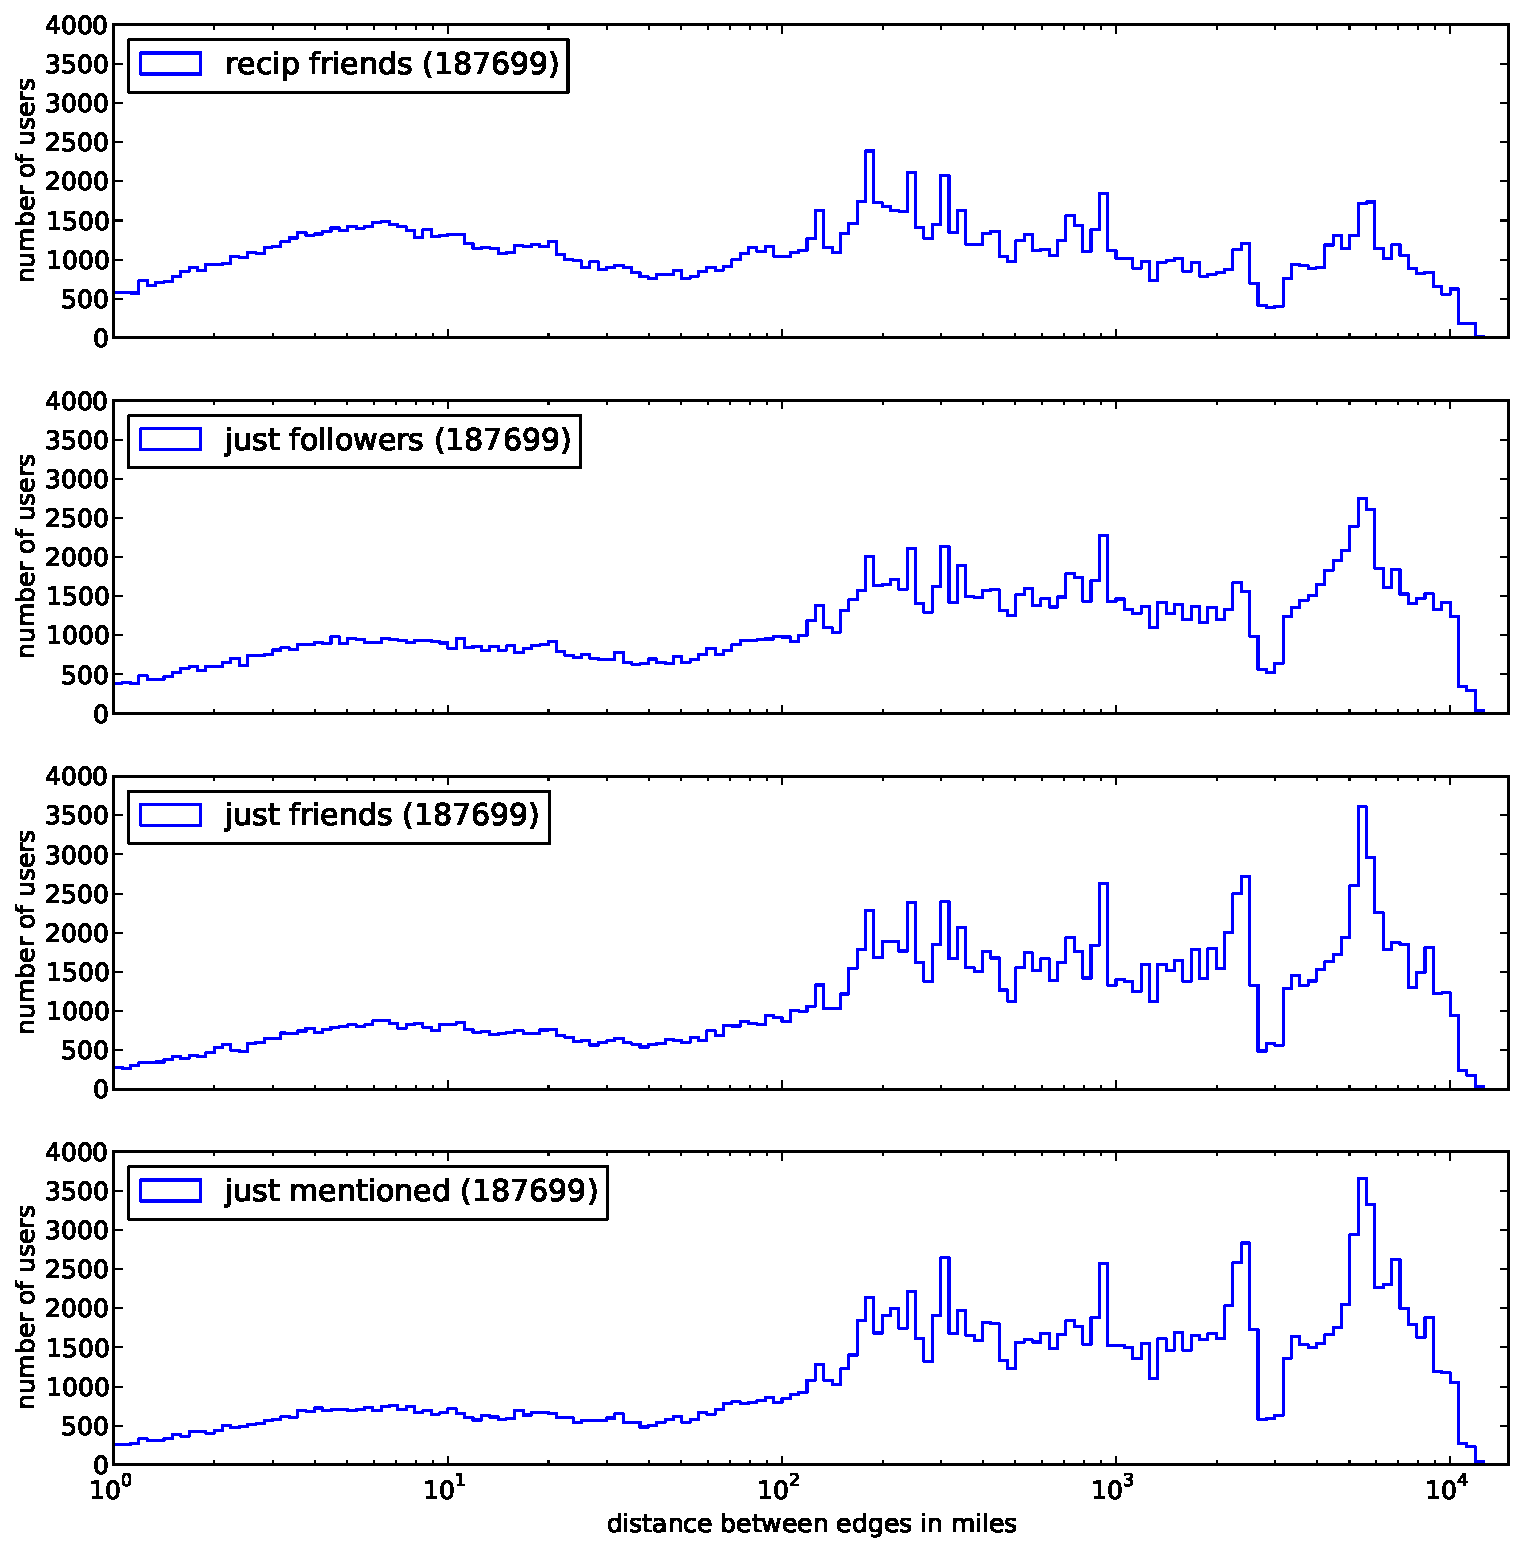
\includegraphics[width=\linewidth]{figures/edge_types_norm.pdf}
\caption{
Histogram of distance to users for different types of relationships.
The curves in this figure are the derivatives of the curves in
Figure~\ref{fig:EdgeTypesCum}.
}
\label{fig:EdgeTypes}
\end{figure}

To understand the distribution of contacts, we created a histogram of the distances between various types of contacts.
We sorted the distances to contacts into 200 logarithmically
scaled bins (40 bins for each power of 10).
Figure~\ref{fig:EdgeTypes} shows the result of plotting the histogram.
%
All four types of contacts follow roughly the same
distribution: one peak around 10 miles from people who live nearby, and several
other peeks between 100 and 10,000 miles. These peeks occur at the distances
between major population centers.

% FIXME: The comment on Twitter being a news distribution network should cite
% that WWW paper from Moon that examines exactly this question.

One reasonable explanation for this is that Twitter is not just a social
network; it is also a news distribution network as described in
\cite{kwak2010why}.
This distribution suggests that users have two types of contacts: people who
they met in real life, and people who they met online or know about via
mainstream media.
%
The former group is useful for predicting location and the latter group is not.
%
In section~\ref{sec:model}, we use this idea that there are two types of
contacts to build a predictive location model based on social ties.


\ifdefined\THESIS
    \begin{figure*}[tb]
    \subsection{Are users closer to people they communicate with?}
    \centering
    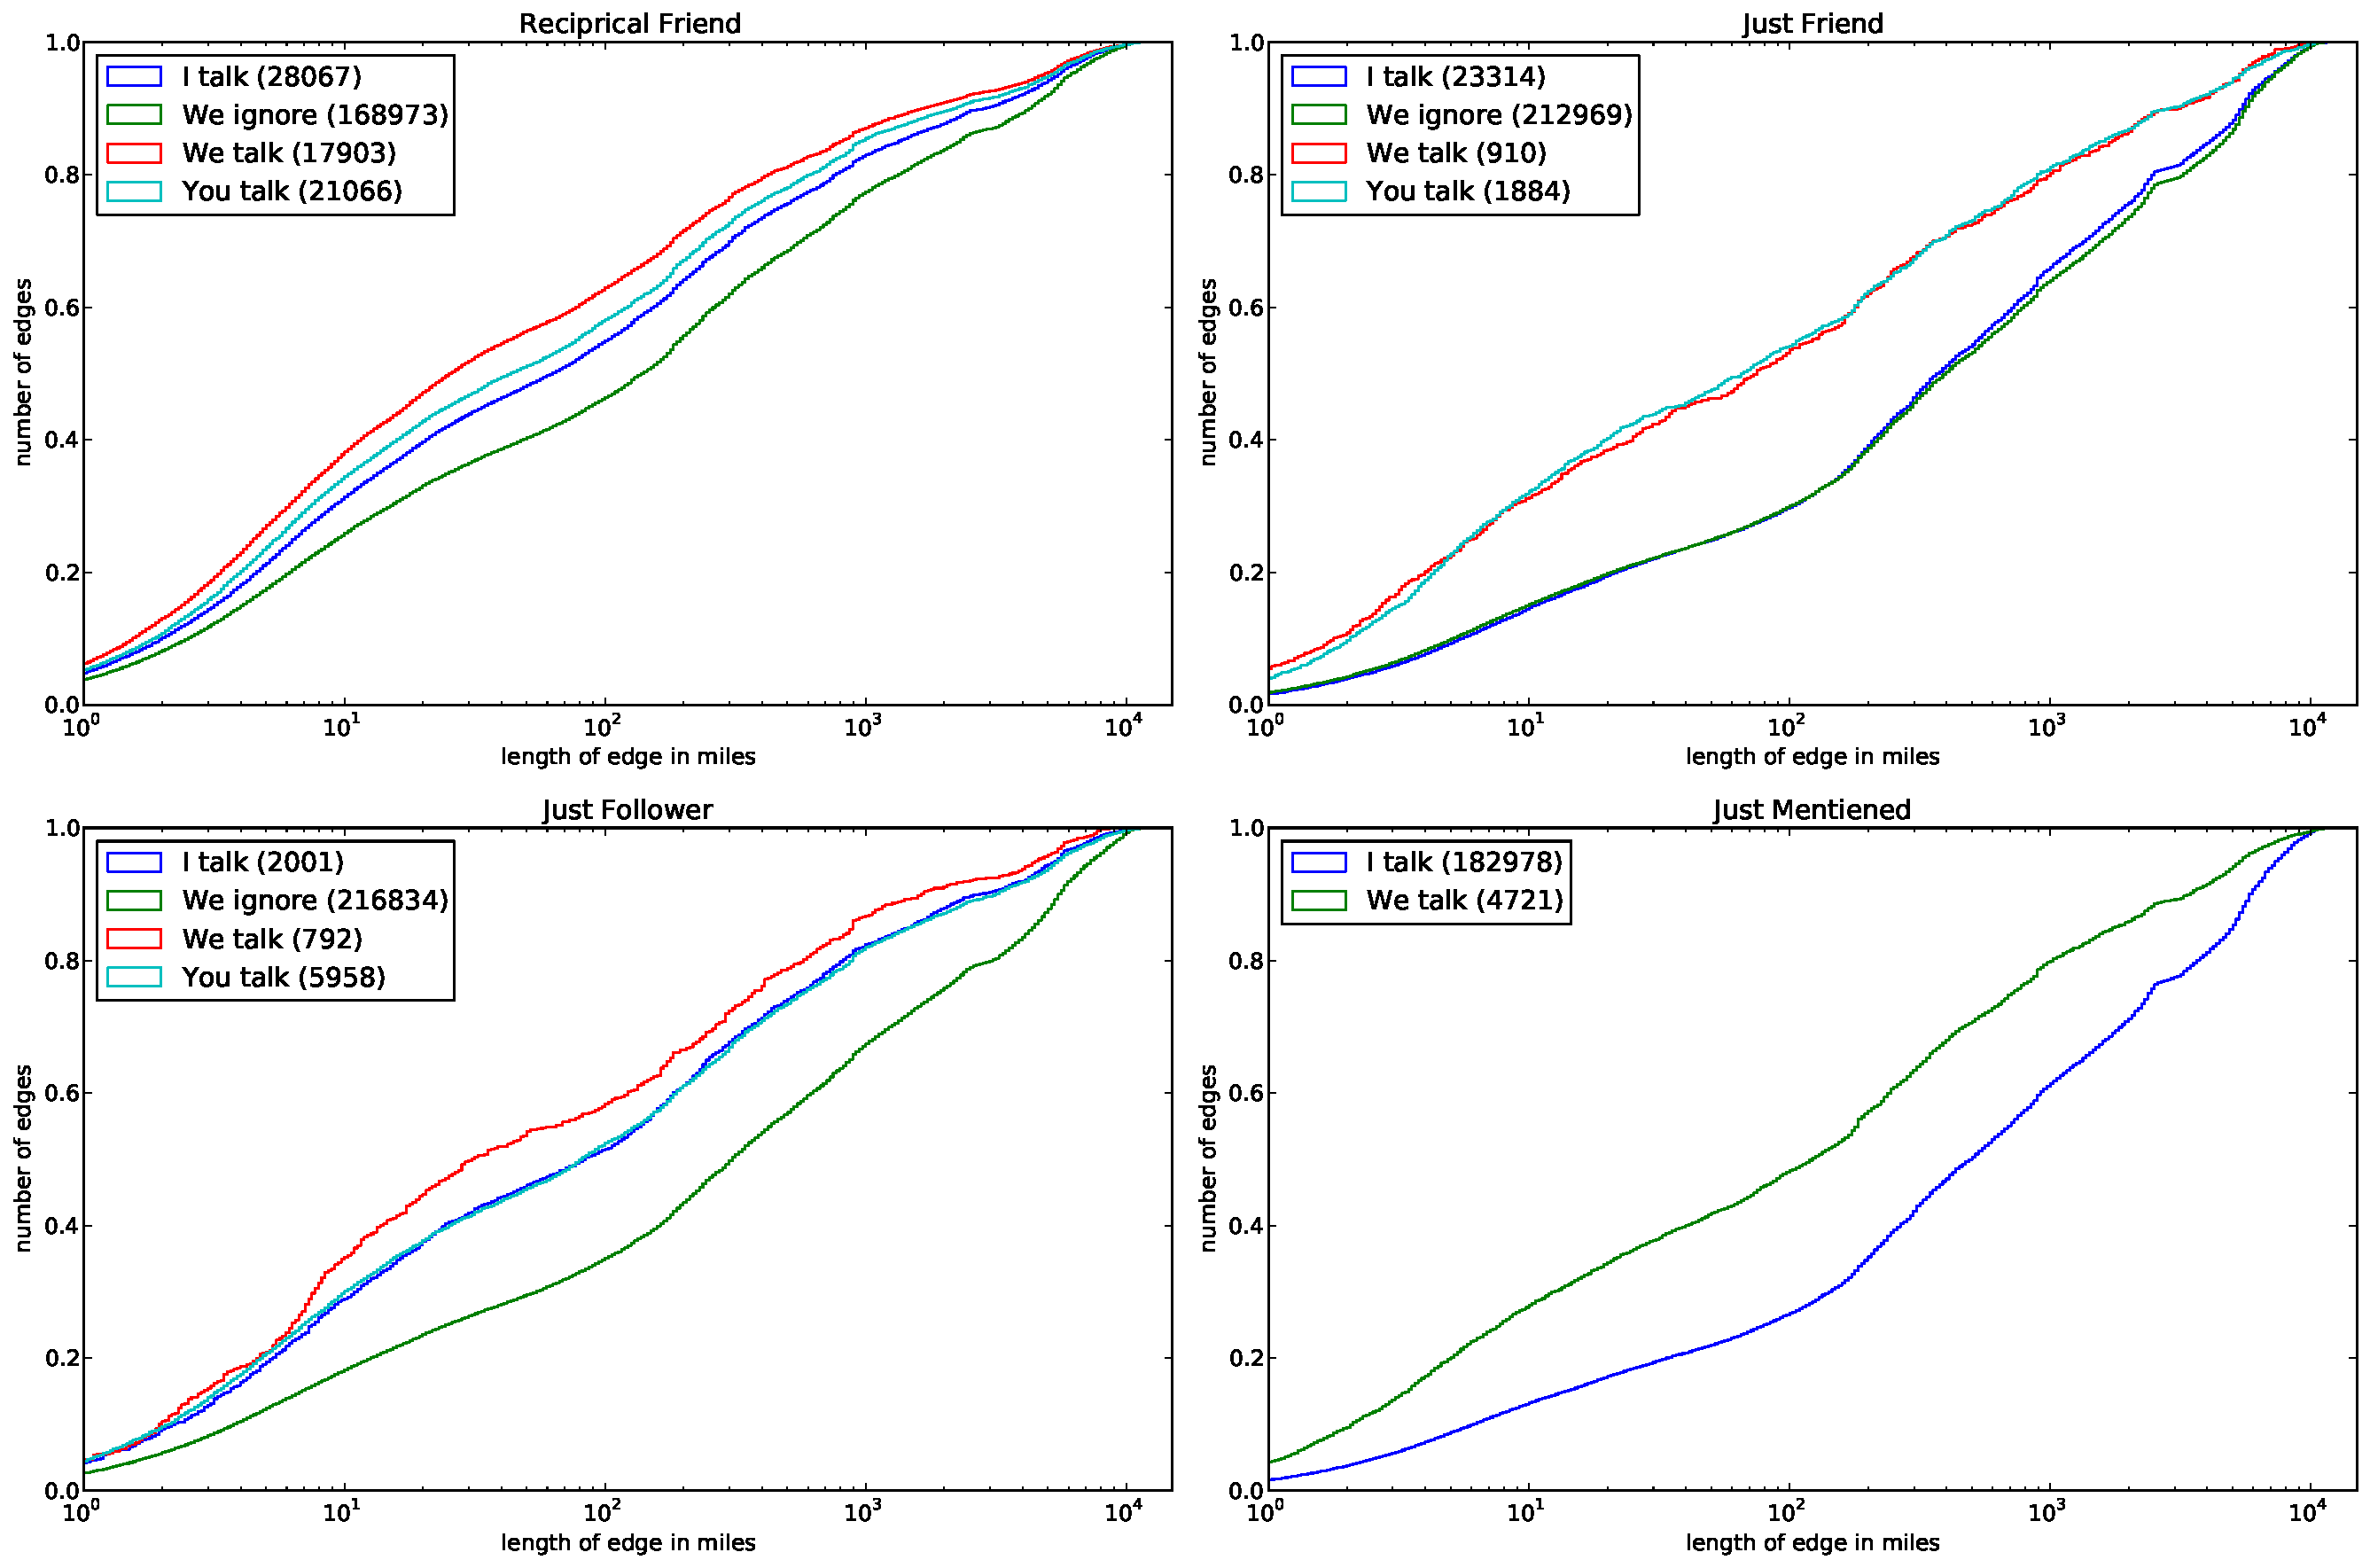
\includegraphics[width=\linewidth]{figures/com_types.pdf}
    \caption{
    CDF of the distance between a geo-located user and various types of contacts
    piloted on a logarithmic scale.
    }
    \label{fig:ComTypes}
    \end{figure*}
\fi

\begin{table*}[tb]
\centering
\begin{tabular}{l | r r | r r | r r | r r}
    & \multicolumn{2}{c}{I Talk}
    & \multicolumn{2}{|c}{We Talk}
    & \multicolumn{2}{|c}{You Talk}
    & \multicolumn{2}{|c}{We Ignore} \\
    \cline{2-9}
    &local&count&local&count&local&count&local&count \\
    \hline
    Just Follower & 40\%&2001 & 47\%&792 & 40\%&5958 & 25\%&216834 \\
    Recip Friend & 42\%&28067 & 50\%&17903 & 45\%&21066 & 35\%&168973 \\
    Just Friend & 21\%&23314 & 40\%&910 & 42\%&1884 & 21\%&212969 \\
    Just Mentioned & 18\%&182978 & 36\%&4721 & & & & \\
\end{tabular}
\caption{
FIXME: explain this
The effect of communication on tie strength.
In these graphs, ``I'' refers to the geo-located user. ``You'' refers to their
contact.
}
\label{tab:ComTypes}
\end{table*}


Table~\ref{tab:ComTypes} shows the relationship between various types of
communication patterns between the geo-located users and their contacts.
In almost every case, increased communication increases the probability that
two users live near each other.
There is one exception: when an average user mentions someone they follow who
does not follow them back, it has no effect.
In other words, if a random user mentions a celebrity who does not bother to
reply, they probably do not live in the same area. This can be seen by the blue
and green lines that are right on top of each other in the Just Friend graph.
On the other hand, in the rare event that someone who is just a friend replies
to their follower, then the probability that they live near each other is much
higher.

The weakest type of contact is for users who were just mentioned, but never
replied to. If the person is mentioned, then 36\% of users with no
friend/follow relationship who have a conversation live within 25 miles.
This is approximately equal to the 35\% of reciprocal friends who ignore each
other and live within 25 miles.
Unsurprisingly, the strongest type of connection is reciprocal friends who
communicate.


\subsection{Are users closer to private accounts?}

\begin{table}[tbh]
\centering
\begin{tabular}{l | r r | r r}
    & \multicolumn{2}{c}{Public}
    & \multicolumn{2}{|c}{Private} \\
    \cline{2-5}
    &local&count&local&count \\
    \hline
    Just Follower & 25\%&204417 & 31\%&21168 \\
    Recip Friend & 37\%&211136 & 41\%&24873 \\
    Just Friend & 21\%&233849 & 39\%&5228 \\
    Just Mentioned & 18\%&183368 & 35\%&4331 \\
\end{tabular}
\caption{
    Private accounts tend to be closer.
}
\label{tab:EdgeTypesProt}
\end{table}

Like many social networks, Twitter allows users to mark their account as
protected. The specifics differ from network to network, but in Twitter's case
a user has to be approved to follow a protected user.
There are demographic differences between public and protected accounts.
For example, Gilbert \cite{gilbert2008network} demonstrates that rural users
are more likely to make their accounts private than public accounts.
In the case of protected accounts on Twitter, basic information
about their profile such as their location and the number of friends and
followers is public, but their friends list, followers list, and the text of
their tweets is private, and not available for analysis.

As seen in Table~\ref{tab:EdgeTypesProt}, the most dramatic difference between
private and public occurs if a user follows a protected account.
%
Since users generally only allow people they know to follow a protected
account, this brings the users almost as close together as if they were
reciprocal friends.
%
On the other hand, if a protected account follows the geo-located user, they
are only slightly more likely to be nearby.

\subsection{If two of your friends live near each other, does that increase the
chance that they live near you?}

\begin{figure}[tb]
\centering
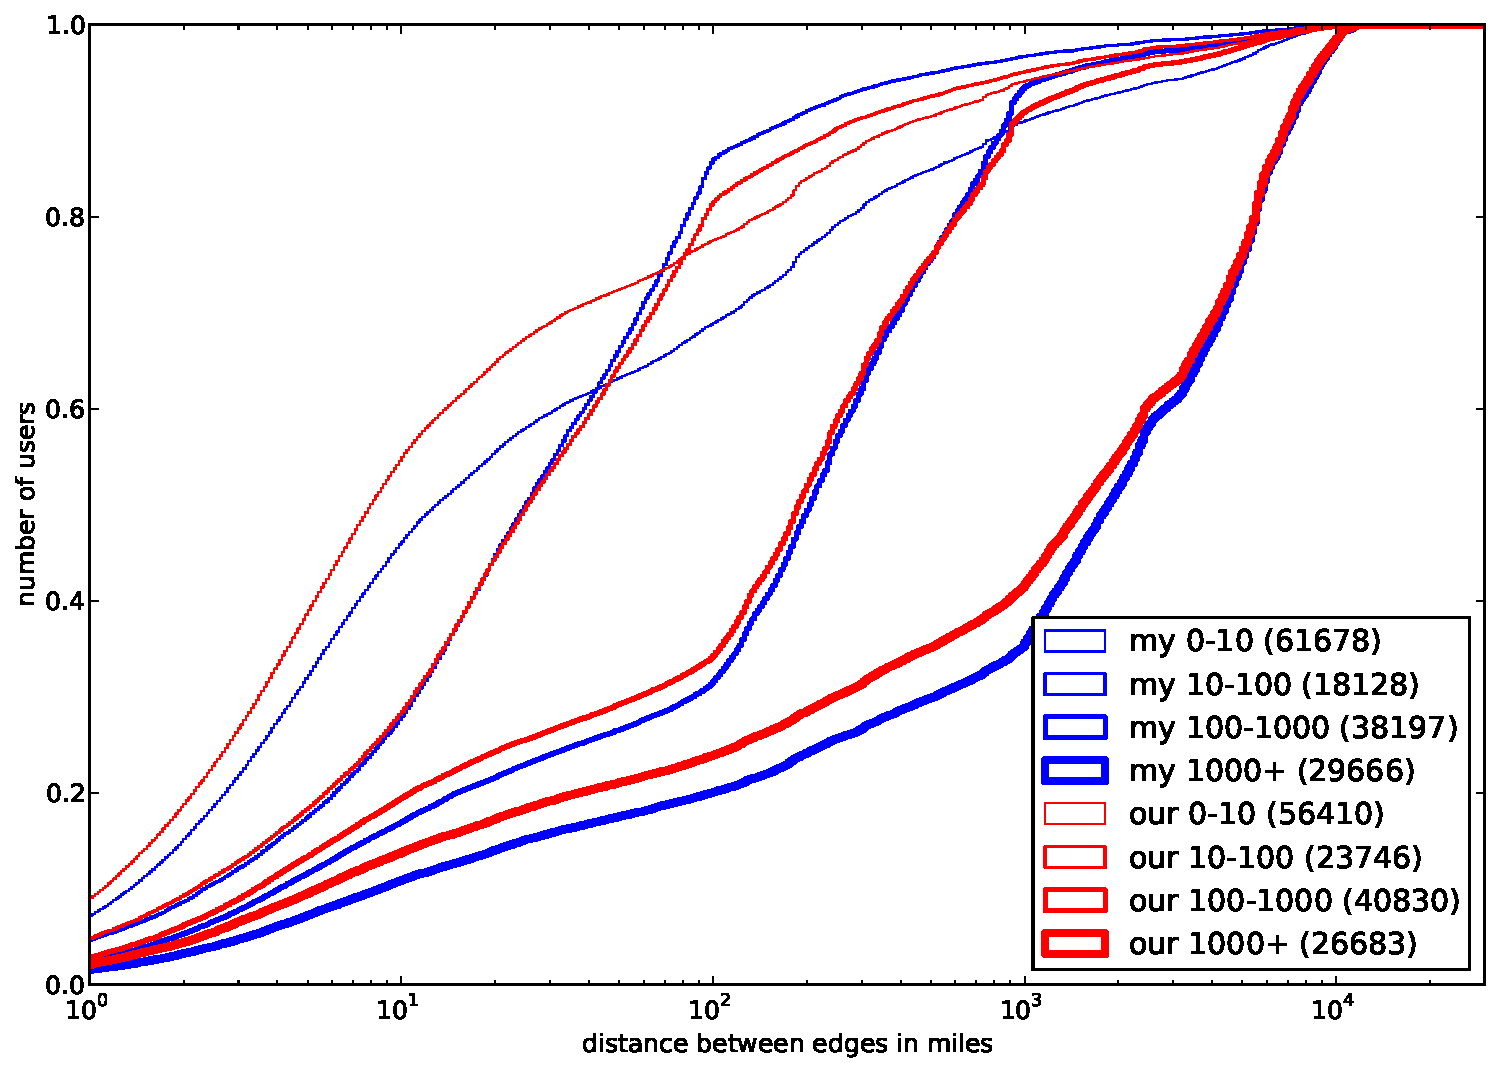
\includegraphics[width=\linewidth]{figures/near_triads.pdf}
\caption{
Comparison between distance to a mutual friend, labeled ``our'', and someone
who is not a mutual friend, labeled ``my''.
The figure in the upper-left corner shows the shape of the social graph we used
to create this graph.
}
\label{fig:NearTriads}
\end{figure}

In this section, we turn our attention to triangles of users.
Finding useful relationships between the edges of a social triangle is tricky
because the three distances depend on each other.
Unfortunately, it is fairly simple to show using the triangle inequality theorem
that if two users are 1000 miles apart, then the third member of the triangle
has to be at least 500 miles from one of the other two.
Since this isn't a useful result, we designed a more complex experiment to
analyze the relationship between the sides of the triangle.
A script searched for a specific pattern in the social network of the
reciprocal friends.  It needed four users who fit the following criteria:
\begin{itemize}
\item ``me'' is the geo-located user
\item ``you'' is reciprocal friends with ``me''
\item ``my'' has no relationship with ``you'' and is reciprocal friends with ``me''
\item ``our'' is reciprocal friends with both ``me'' and ``you''
\end{itemize}

% FIXME: when you talk about the me, you, my, our. I would put that subfigure
% from the figure in the body of the text so it is clearer. And the language
% itself is pretty tough to follow. Not sure on how to improve it, but it is
% confusing.

We found this pattern for 147669 of the geo-located users.
If a user had multiple instances of this pattern, it picked one of them
randomly so that particular users would not bias the results.
Since our crawler only retrieved friend and follower information for at most
seven reciprocal friends per user, it is reasonable to assume that this pattern
is much more common, but the sample is more than enough data to draw some
conclusions.

Figure~\ref{fig:NearTriads} shows a comparison between the ``my'' users and the
``our'' users.
For each of the ``my'' users and the ``our'' users, we put them into one of
four logarithmically scaled bins based on their distance from the ``you'' user.
Then we plot the CDF for the distance to ``me'' for each user in the set. This
allows us to investigate the effect of mutual friendship on distance.
We report one very simple result: if two of your friends are close (within 10
miles), then whether they know each other or not is strongly affects how close
you are to them. If they are farther apart, it doesn't matter.

\subsection{Does the number of friends and followers a person have affect how
close they are?}

\begin{figure*}[tb]
\centering
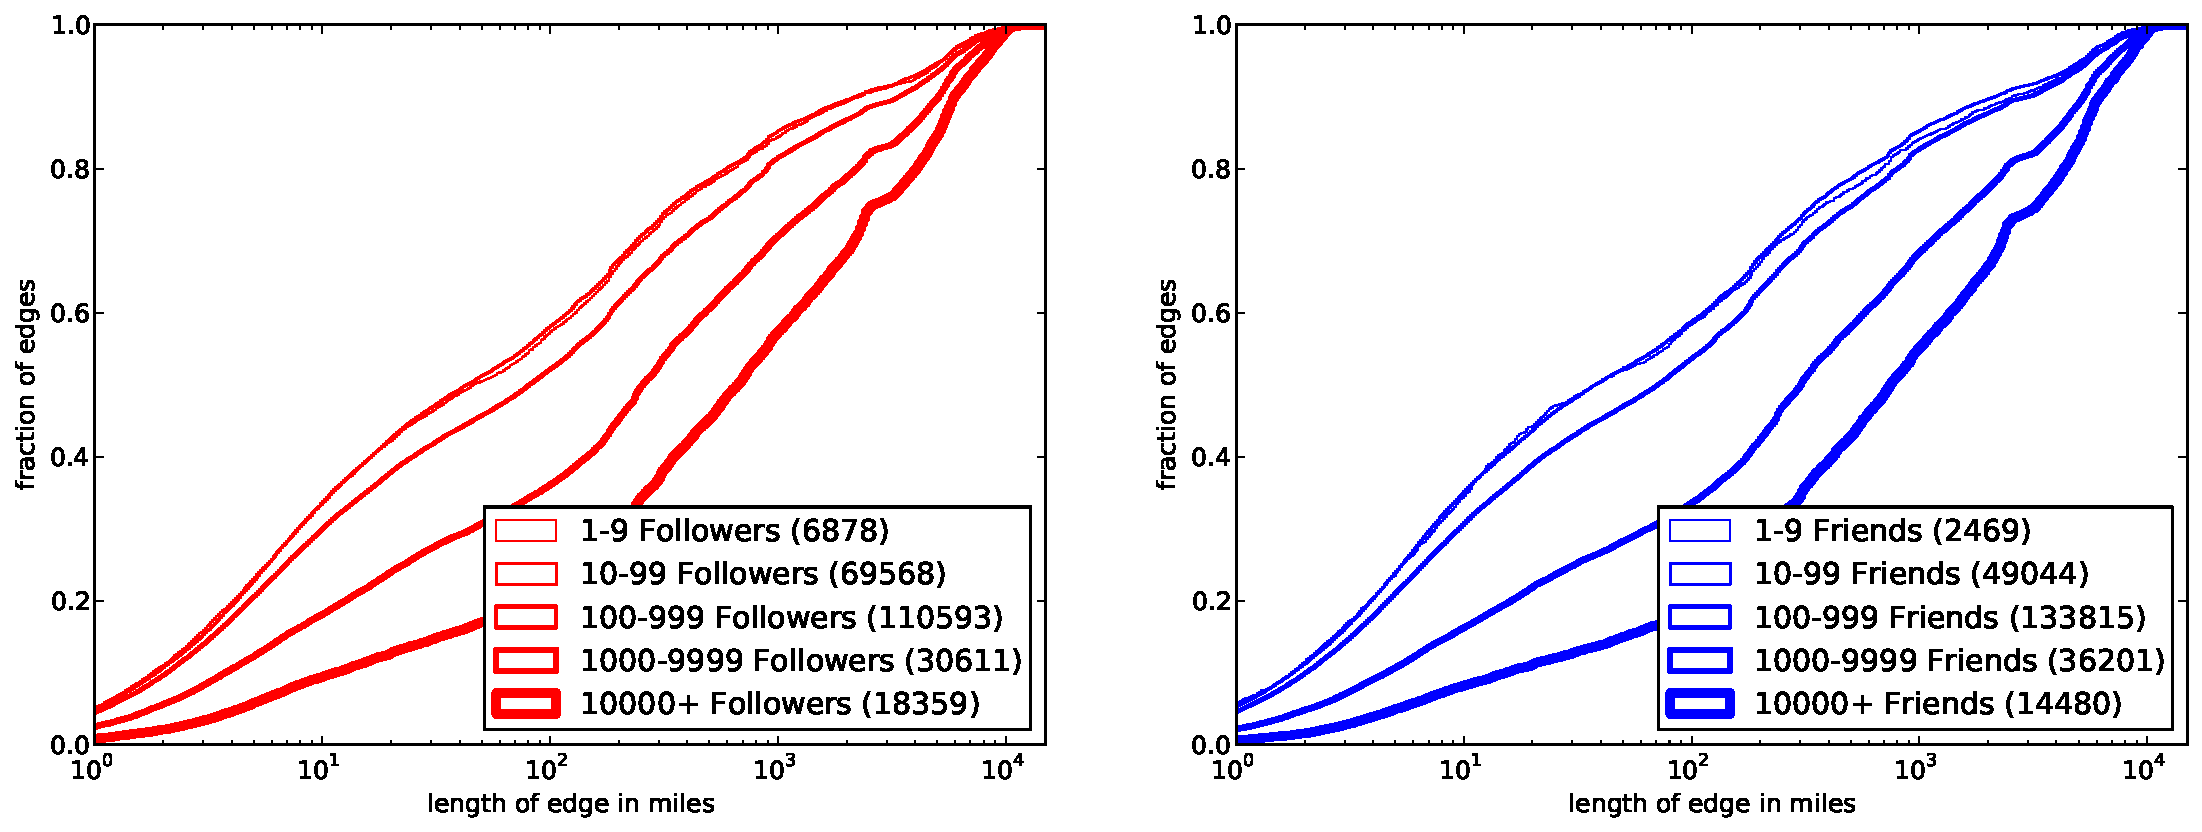
\includegraphics[width=\linewidth]{figures/edge_counts.pdf}
\caption{
A comparison between number of followers and proximity---people who have more
friends or followers tend to be further away.
}
\label{fig:EdgeCounts}
\end{figure*}

%FIXME: this is important: should we move it up?

Since the primary goal of this research is to predict the location of users, we
focus our attention on the number of friends and followers a contact has rather
than the numbers for the geo-located user.
We took each of the reciprocal friendships what we looked at in
Section~\ref{sec:EdgeTypes} and put them into log-scaled bins based on their
number of friends or followers that the contact had.
Figure~\ref{fig:EdgeCounts} shows the result of this procedure.

In general, people who are more promiscuous followers and friends are less
likely to live nearby. This makes sense because it is easy to meet 5 Twitter
users in real life, but very few people know 500 Twitter users who live in the
same town.

Mainstream media and celebrity accounts such as the New York Times and Lady
Gaga have millions of followers while normal users rarely have more than a few
hundred.
Follower count is a good way to distinguish celebrity and news accounts which
are useless for location prediction.

\subsection{Are some users closer to all of their friends and followers?}

\begin{figure}[tb]
\centering
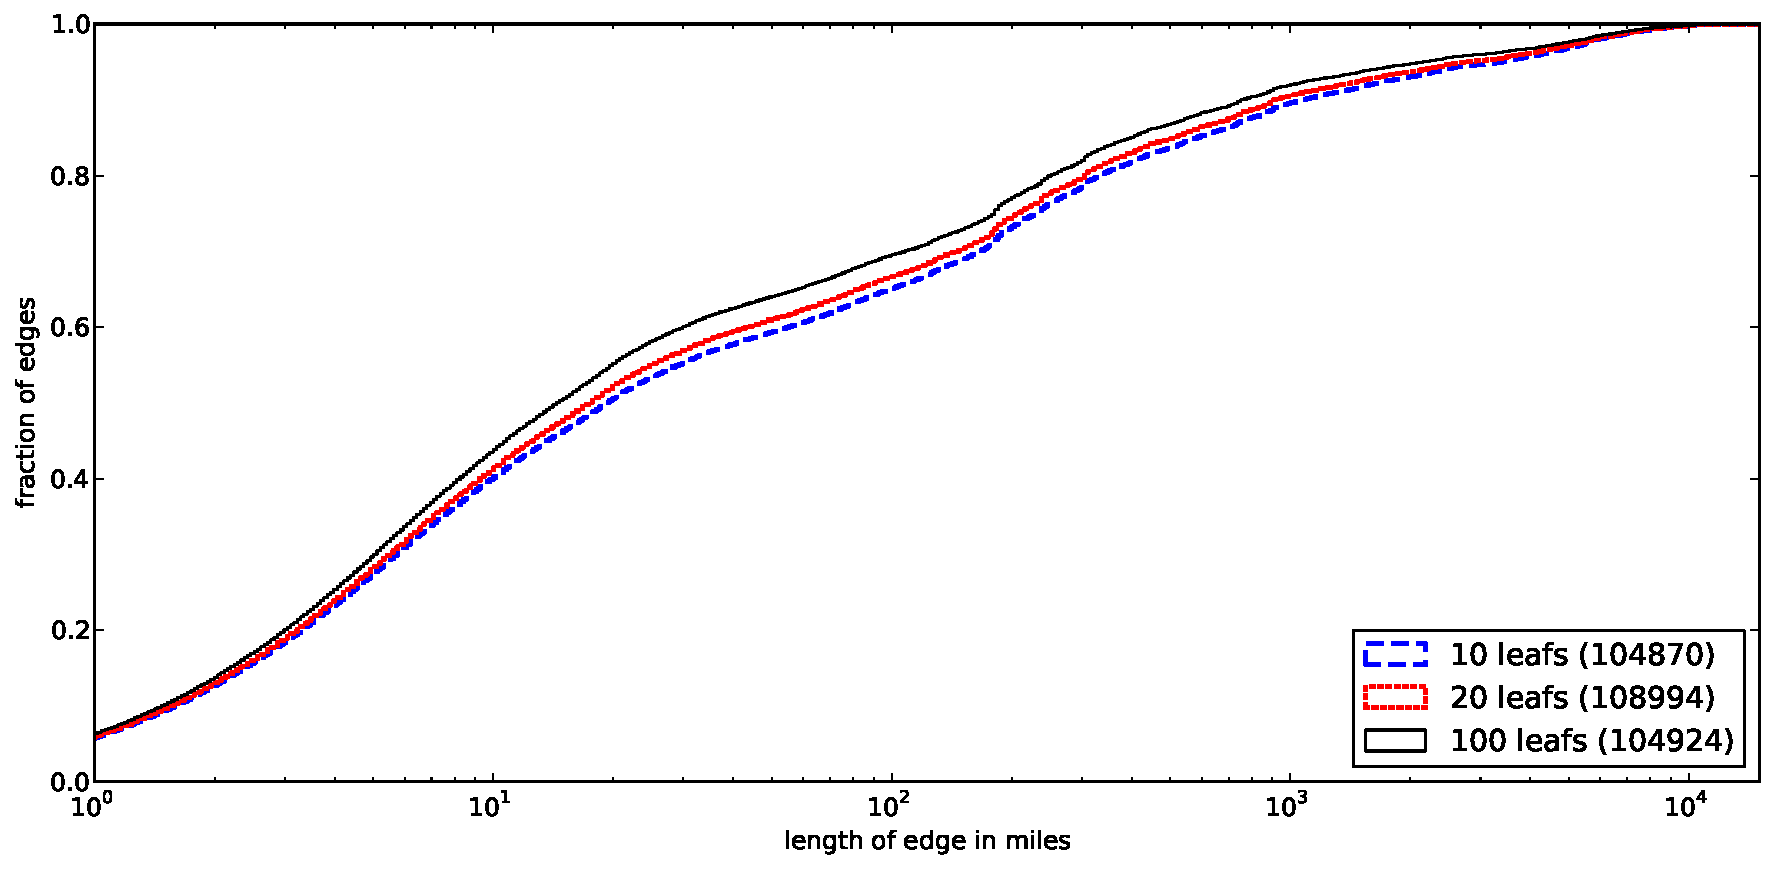
\includegraphics[width=\linewidth]{figures/locals_cmp.pdf}
\caption{
    FIXME: caption
}
\label{fig:LocalCmp}
\end{figure}

\begin{figure}[tb]
\centering
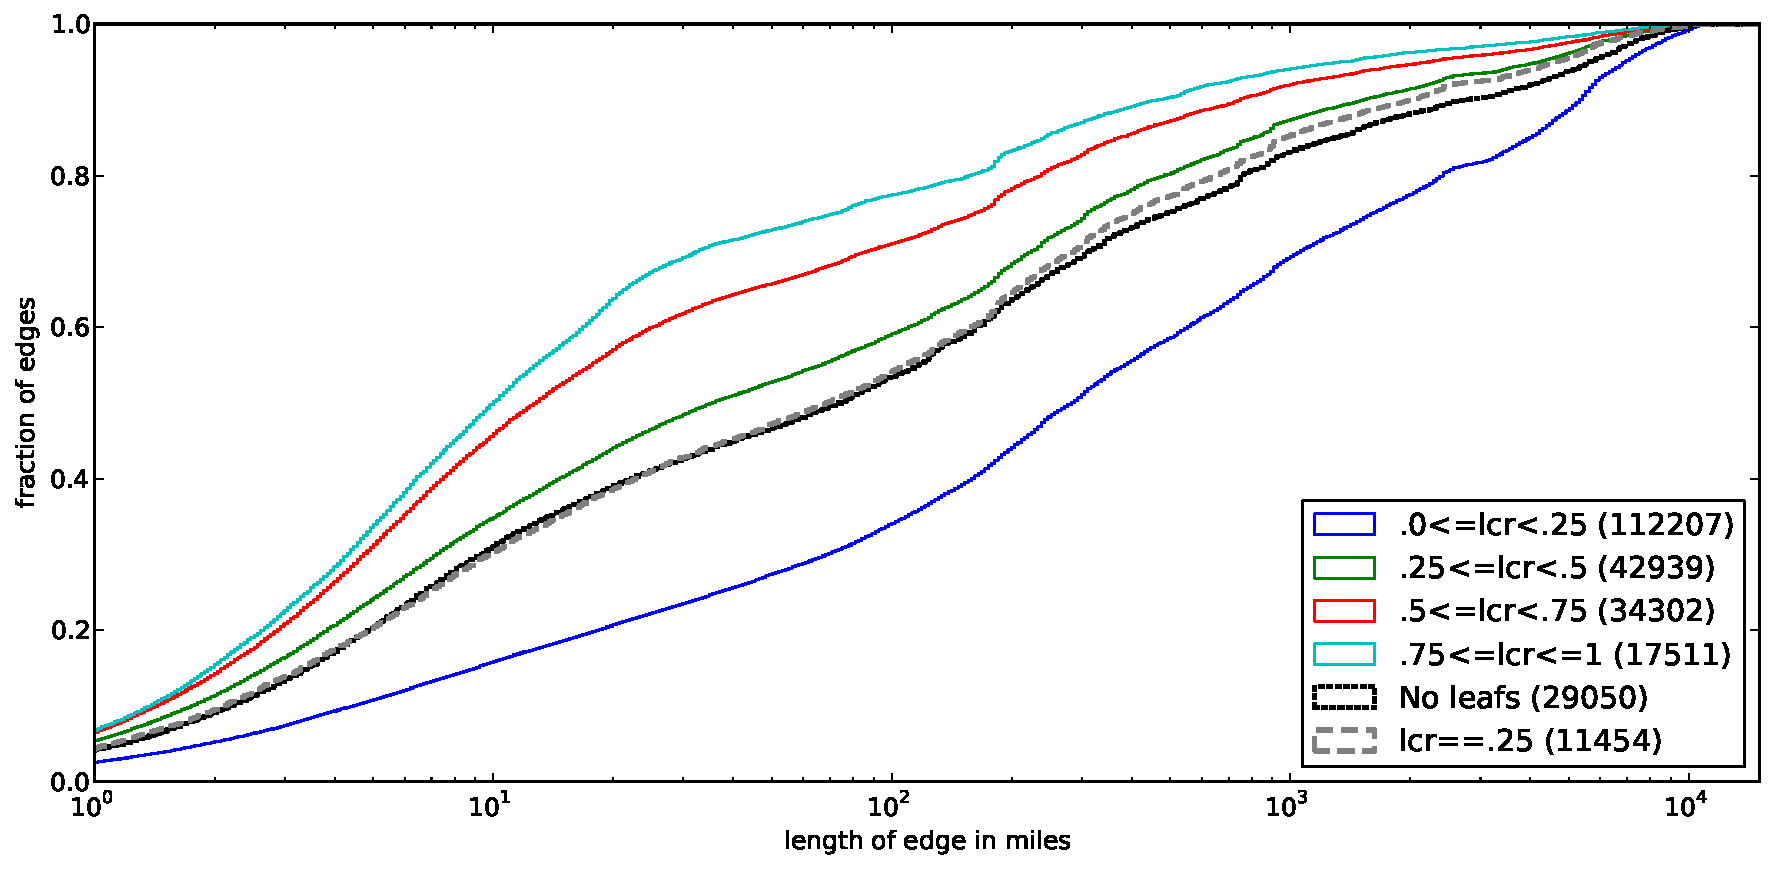
\includegraphics[width=\linewidth]{figures/locals_10.pdf}
\caption{
The colored lines show the distance to contacts split into groups based on the
proportion of the contact's friends and followers who live near the contact.
The dotted line shows the distance to contacts who have no locatable contacts.
}
\label{fig:Local10}
\end{figure}

In the previous sections we only looked at the contacts of the geo-located
users. In this section we will go two steps out on the social graph and
investigate the friends-of-friends.
%
For each of the contacts we calculated the distance to at most fifty followers.
%
\textbf{Local Contact Ratio} is the fraction of those followers who lived within 25 miles
of the contact.
% FIXME: update this with the new graphs
%
Around one in ten contacts did not have any followers with a location they were
treated as a separate group.
%
We repeated this procedure on the contacts' friends to produce
Figure~\ref{fig:EdgeCounts}.

The figure shows that some users are much more local than other users.
For example, a local newspaper may have thousands of followers and few friends,
but the people who follow a newspaper are generally local.
According to the other factors we looked at, the newspaper is a bad predictor
of location, but in reality it is a great predictor.

Of the factors we have investigated, this is the most strongly correlated with
distance.
One problem with this technique is that it is somewhat expensive to deal with
the profiles two steps out on the social graph.
It may be possible to achieve similar results by visiting fewer
friends-of-friends.
